% Modelo Lógico do Banco de Dados - Pollen
\begin{figura}{Modelo Lógico do Banco de Dados - Estrutura física das tabelas}{O Autor}
\centering
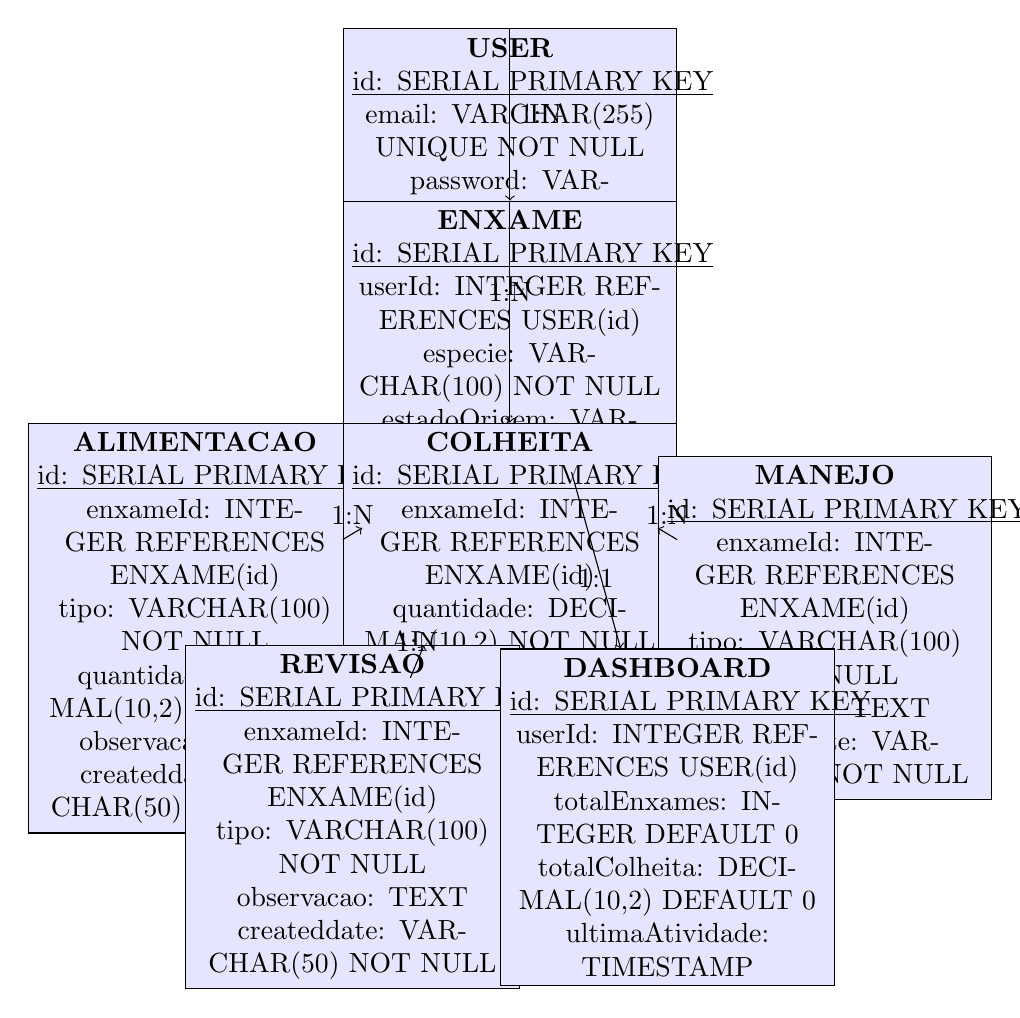
\begin{tikzpicture}[scale=0.8]
% Definição de estilos
\tikzset{
  table/.style={rectangle, draw, fill=blue!10, text width=4cm, text centered, minimum height=2cm},
  pk/.style={rectangle, draw, fill=red!20, text width=3.8cm, text centered, minimum height=0.3cm},
  fk/.style={rectangle, draw, fill=yellow!20, text width=3.8cm, text centered, minimum height=0.3cm},
  field/.style={rectangle, draw, fill=white, text width=3.8cm, text centered, minimum height=0.3cm}
}

% Tabela USER
\node[table] (user_table) at (0,9) {\textbf{USER}\\
\underline{id: SERIAL PRIMARY KEY}\\
email: VARCHAR(255) UNIQUE NOT NULL\\
password: VARCHAR(255) NOT NULL\\
planType: VARCHAR(50) DEFAULT 'FREE'\\
status: VARCHAR(20) DEFAULT 'pending'\\
createdAt: TIMESTAMP DEFAULT NOW()};

% Tabela ENXAME
\node[table] (enxame_table) at (0,6) {\textbf{ENXAME}\\
\underline{id: SERIAL PRIMARY KEY}\\
userId: INTEGER REFERENCES USER(id)\\
especie: VARCHAR(100) NOT NULL\\
estadoOrigem: VARCHAR(50) NOT NULL\\
localizacao: VARCHAR(255) NOT NULL\\
identificador: VARCHAR(50) NOT NULL\\
forcaEnxame: VARCHAR(20) NOT NULL};

% Tabela ALIMENTACAO
\node[table] (alimentacao_table) at (-5,3) {\textbf{ALIMENTACAO}\\
\underline{id: SERIAL PRIMARY KEY}\\
enxameId: INTEGER REFERENCES ENXAME(id)\\
tipo: VARCHAR(100) NOT NULL\\
quantidade: DECIMAL(10,2) NOT NULL\\
observacao: TEXT\\
createddate: VARCHAR(50) NOT NULL};

% Tabela COLHEITA
\node[table] (colheita_table) at (0,3) {\textbf{COLHEITA}\\
\underline{id: SERIAL PRIMARY KEY}\\
enxameId: INTEGER REFERENCES ENXAME(id)\\
quantidade: DECIMAL(10,2) NOT NULL\\
tipo: VARCHAR(100) NOT NULL\\
observacao: TEXT\\
createddate: VARCHAR(50) NOT NULL};

% Tabela MANEJO
\node[table] (manejo_table) at (5,3) {\textbf{MANEJO}\\
\underline{id: SERIAL PRIMARY KEY}\\
enxameId: INTEGER REFERENCES ENXAME(id)\\
tipo: VARCHAR(100) NOT NULL\\
descricao: TEXT\\
createddate: VARCHAR(50) NOT NULL};

% Tabela REVISAO
\node[table] (revisao_table) at (-2.5,0) {\textbf{REVISAO}\\
\underline{id: SERIAL PRIMARY KEY}\\
enxameId: INTEGER REFERENCES ENXAME(id)\\
tipo: VARCHAR(100) NOT NULL\\
observacao: TEXT\\
createddate: VARCHAR(50) NOT NULL};

% Tabela DASHBOARD
\node[table] (dashboard_table) at (2.5,0) {\textbf{DASHBOARD}\\
\underline{id: SERIAL PRIMARY KEY}\\
userId: INTEGER REFERENCES USER(id)\\
totalEnxames: INTEGER DEFAULT 0\\
totalColheita: DECIMAL(10,2) DEFAULT 0\\
ultimaAtividade: TIMESTAMP};

% Relacionamentos
\draw[->] (user_table) -- node[right] {1:N} (enxame_table);
\draw[->] (enxame_table) -- node[above] {1:N} (alimentacao_table);
\draw[->] (enxame_table) -- node[above] {1:N} (colheita_table);
\draw[->] (enxame_table) -- node[above] {1:N} (manejo_table);
\draw[->] (enxame_table) -- node[above] {1:N} (revisao_table);
\draw[->] (user_table) -- node[below] {1:1} (dashboard_table);

\end{tikzpicture}
\label{fig:modelo-logico-banco}
\end{figura}